\rt{Make sure to double-check the cfp. I see no Supplemental Material Statement for example.}

\section{Introduction}
\sepfootnotecontent{sf:webID}{
    \url{https://www.w3.org/wiki/WebID}
}
\sepfootnotecontent{sf:dataSovereignty}{
    \url{https://digital-strategy.ec.europa.eu/en/policies/strategy-data}
}

Data sovereignty seeks to establish a more just definition of personal data ownership in terms of data usage and storage.
It can be defined as ``the self-determination of individuals and organizations with regard to the use of their data''~\cite{verstraete2022solid},
which in practice can be interpreted as the power to choose where one's data is stored and who has access to it~\cite{verstraete2022solid}.
Multiple studies have denoted problems of ownership, democracy, reinforcement of inequality, and antagonism between users and owners of social web applications~\cite{Terranova2000FreeLP, Curran2016ch1, Sevignani2013, 9663788}.
Several authors consider decentralizing web data an insufficient solution~\cite{9663788, Curran2016ch1}; yet, it is an integral component of initiatives focused on data sovereignty,
which necessitates technical research.
Linked Data can be considered a technical contribution toward the development of a decentralized web.
It supports the creation of Decentralized Knowledge Graphs (DKGs) through the use of dereferenceable IRIs.
These IRIs allow access to additional Knowledge Graphs (KGs) containing information relevant to what an IRI identifies.
For example, a WebID~\sepfootnote{sf:webID} represents an agent, dereferencing it can provide the name of the user, among other information, without having to store the information locally.
Despite these advantages, SPARQL query processing is predominantly carried out in centralized environments, partially due to a more established understanding of how to optimize queries in such settings.

Link Traversal Query Processing (LTQP)~\cite{Hartig2012} is a query paradigm designed for querying unindexed, decentralized environments by leveraging the descriptive power of IRI dereferencing.
LTQP involves recursively dereferencing IRIs discovered in a query engine's internal triple store during query execution to expand its base of information.
The main difficulty of LTQP is the large domain of exploration, which leads to a high number of HTTP requests as demonstrated by \citeauthor{hartig2016walking}~\cite{hartig2016walking}.
From another perspective, and without contradicting \citeauthor{hartig2016walking}~\cite{hartig2016walking}, \citeauthor{Taelman2023}~\cite{Taelman2023} have demonstrated that in Decentralized Environments with Structural Properties (DESPs), it is possible to attain query completeness for various types of practical queries within acceptable execution times for the context of social media applications~\cite{nielsen1993response}.
%Moreover, they showed that query planning could significantly influence the execution time.
Structural properties ensure data discoverability, which in turn helps guarantee result completeness.
In practice, DESPs emerge in various contexts, such as social networks~\cite{Taelman2023} and the publication of sensor data~\cite{tam_iswc_traversalsensortree_2024}, among others.
%Concrete DESPs has been shown to be beneficial for datasets following the Solid protocol~\cite{Taelman2023} and the TREE specification~\cite{tam_iswc_traversalsensortree_2024}.
The work of \citeauthor{Taelman2023}~\cite{Taelman2023} suggests that various optimizations are feasible for LTQP in decentralized environments that exhibit structural properties.
This contrasts with the more pessimistic conclusion of \citeauthor{hartig2016walking}~\cite{hartig2016walking}, whose study of LTQP over Open Linked Data found limited opportunities for optimization, primarily due to the HTTP request bottleneck.

In general, the World Wide Web lacks a structure that query engines can exploit for optimization.  
This is because any document can be published anywhere, with no standard index or trust mechanism to guide discovery.  
However, within specific \emph{subwebs}, defined as subsections of the web controlled by particular data providers, implicit or explicit data structures may emerge, which query engines can leverage.
In this work, we extend a dataset summarization approach for decentralized environments known as the \emph{shape index}\ifanonymous~\cite{tam2024opportunitiesshapebasedoptimizationlinkAnon}\else~\cite{tam2024opportunitiesshapebasedoptimizationlink}\fi.
We apply this approach to enable link pruning within LTQP, removing links that are not relevant to the query, based on an analysis of RDF data shapes and the user's query.
The analysis is performed by conducting a query-shape subsumption check to determine whether a resource conforming to a given shape is relevant to a query.
Our approach assumes a DKG composed of subwebs, each hosted by data providers and containing shape indexes.  
To illustrate this, we present the example shown in Figure~\ref{fig:dkg}, which features a network of three subwebs, each with its own shape index, as well as resources located outside the subwebs.
The query executed by the engine aims to retrieve posts from subweb 3, along with all their replies.  
Our pruning solution allows the engine to explore only the relevant parts of the network, guided by the shapes associated with the resources and the structure of the query.
The process begins with the query engine dereferencing the shape index of subweb 3 and performing a query-shape subsumption check, which determines that only the post from this subweb needs to be accessed.  
It then checks the shape index of subweb 1, where the subsumption check reveals no resources relevant to the query.  
Next, it examines the shape index of subweb 2 and identifies that only comments (i.e., replies) are relevant.  
Finally, the engine dereferences all reachable resources outside the subwebs that are linked to these relevant comments.

\begin{figure}
   \centering
   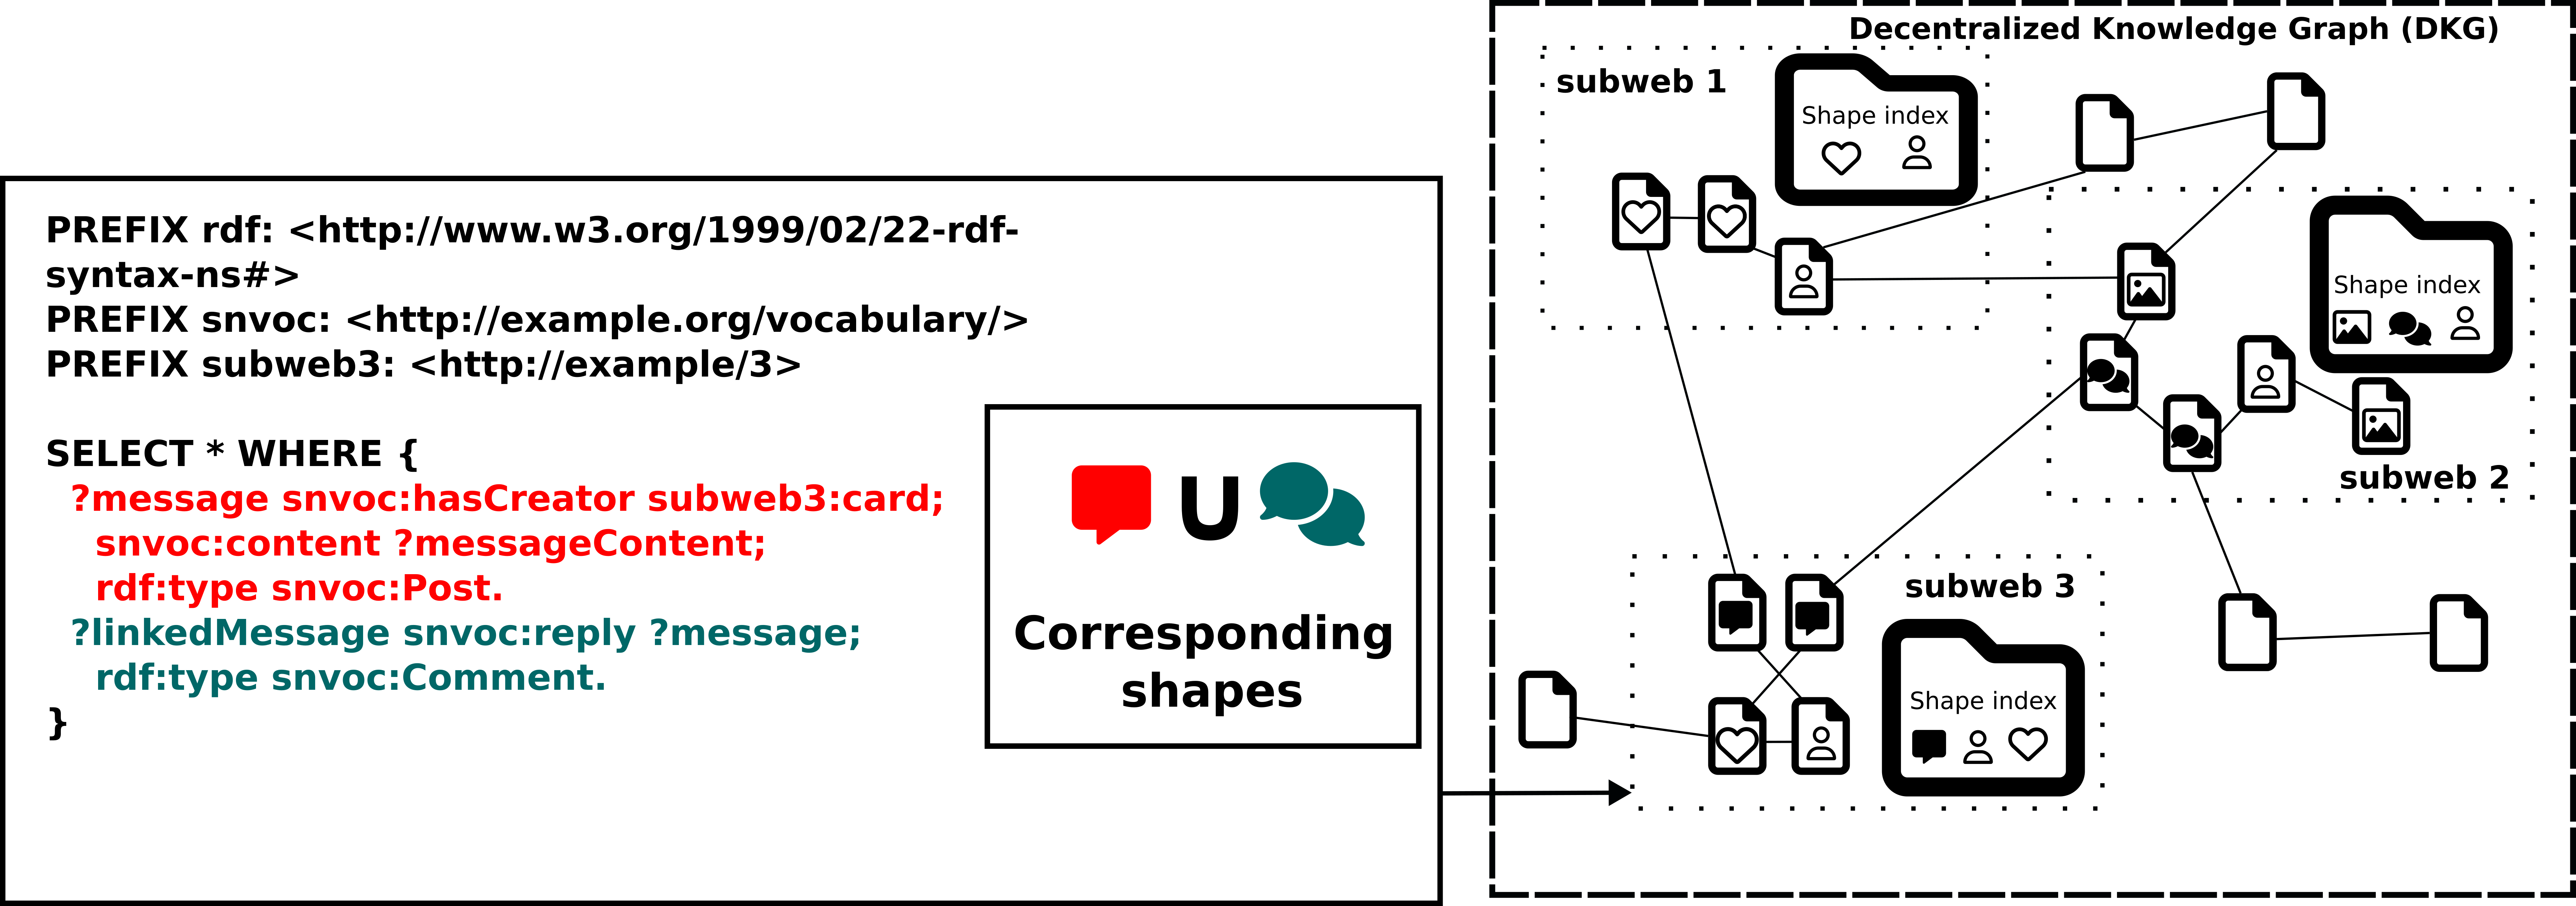
\includegraphics[width=0.70\textwidth]{figure/dkg.png}
   \caption{
      Given that the resources of a DKG are indexed with a shape index, a query engine can dereference a subset of the network.
      The nodes represent RDF resources, while the edges represent IRIs linking one resource to another (see Section \ref{sec:dkg}).
      Each subweb has a shape index that maps shapes, represented by icons, to RDF resources by embedding the icon within the node.
      The query engine starts its query at subweb 3, and the relevant query resources in a subweb are identified with a black node.
    }
    \label{fig:dkg}
\end{figure}

This paper presents our link pruning approach using shape indexes, along with a query-shape subsections algorithm to assess the relevance of data sources, and experimental results based on a synthetic benchmark.

\iffalse
This paper is organized as follows: first, we discuss the \hyperref[sec:related_work]{related work} and present \hyperref[sec:preliminaries]{preliminaries}.
We then describe our \hyperref[sec:approach]{approach}, we then introduce the \hyperref[sec:problem_statement]{problem statement}, followed by the \hyperref[sec:experiment]{experimental setup} and the \hyperref[sec:result]{discussion of results}.
Finally, we conclude the article.
\fi